\chapter{Graphiques et géométrie}\label{graph}

\section{Différentes méthodes }

$\star$ Le package \jargon{pstricks} a été longtemps très largement utilisé pour réaliser des figures géométriques et graphiques.

Il l'est toujours actuellement et offre de nombreuses possibilités pour créer des graphiques et figures géométriques.

Cependant, on rencontre des problèmes de compatibilité lorsque l'on compile en PDF\LaTeX{}.

$\star$ Le programme \jargon{metapost} est également très puissant et offre de nombreuses possibilités. 

Cependant il génére des fichiers externes qu'il faut ensuite inclure au document.

$\star$ Mon choix s'est donc porté sur le package \jargon{TikZ} qui possède un très grand nombre d'options et de possibilités, ainsi que sur un dérivé, le package \jargon{TkZ} qui utilise le premier et offre une syntaxe simplifié dans pas mal de cas de figures.

\section{Présentation générale de TikZ et TkZ}

Les packages \jargon{TikZ} et \jargon{TkZ} possèdent des librairies . 

Pour les utiliser il faut ajouter dans le préambule :

\verb!\usepackage{tikz,tkz-base,tkz-fct,tkz-euclide,tkz-tab,tkz-graph,tikz-3dplot}!

\begin{verbatim}
\usetikzlibrary{calc,shapes,arrows,plotmarks,lindenmayersystems,decorations,
decorations.markings,decorations.pathmorphing,
decorations.pathreplacing,patterns,positioning,decorations.text}
\end{verbatim}!

Pour utiliser les différents objets \jargon{TkZ}, on ajoute :

\verb!\usetkzobj{all}!

Certaines commandes \jargon{TkZ} nécessite d'effectuer des calculs pour obtenir les figures et graphiques et utilise le package \jargon{pgfplots}.

On ajoute donc également la commande 
\verb!\usepackage{pgfplots}!

On ajoutera enfin l'appel au package \jargon{etex} qui augmente la capacité de mémoire de \LaTeX{}, ce qui peut s'avérer nécessaire lorsque le document contient pas mal de figures nécessitant beaucoup de calculs.

Voici donc un préambule possible tenant compte de tous ces \jargon{packages} :

\medskip

\VerbatimInput[label={[Document TikZ]},gobble=0]{exemples/doctikz.tex}

\medskip

\section{Exemples de figures utilisant TikZ}

\begin{info}
Ces figures sont réalisables avec des commandes des \jargon{packages} \ordi{TkZ} que l'on voit juste après.
\end{info}


\medskip

\VerbatimInput[label={[Axe gradué]},gobble=0]{exemples/tikzaxegradue.tex}

\medskip
\begin{center}
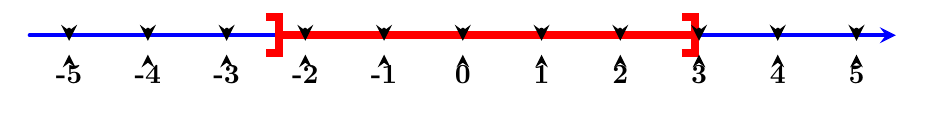
\begin{tikzpicture}[scale=1,line cap=round,line join=round,x=1.0cm]
\draw[>=stealth,->,line width=1.5pt,color=blue] (-5.5,0) -- (5.5,0);
\draw[{]-]},line width=3pt,color=red] (-2.5,0) -- (3,0);
\foreach \x in {-5,...,5}
\draw[color=black,line width=1.5pt] (\x,2pt) -- (\x,-2pt);
\foreach \x in {-5,...,5}
\draw (\x,-7pt) node[below,font=\bfseries] {\x};
\end{tikzpicture}
\end{center}
\medskip

\VerbatimInput[label={[Courbe passant par des points donnés]},gobble=0]{exemples/tikzcourbepoints.tex}

\medskip
\begin{center}
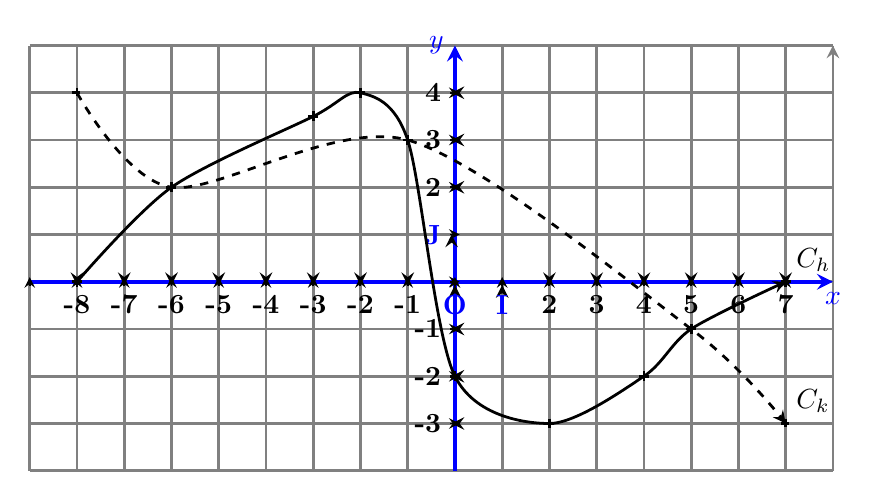
\begin{tikzpicture}[scale=0.6,>=stealth]
            \draw[gray] (-9,-4)grid(8,5);
            \draw[->,line width=1.5pt,color=blue] (-9,0)--(8,0)node[below] {$x$};
            \foreach \x in {-8,-7,-6,-5,-4,-3,-2,-1,2,3,4,5,6,7}
\draw[color=black] (\x,2pt) -- (\x,-2pt) node[below,font=\bfseries] {\x};
            \draw[->,line width=1.5pt,color=blue] (0,-4)--(0,5)node[left] {$y$};
            \foreach \y in {-3,-2,-1,2,3,4}
\draw[color=black] (2pt,\y) -- (-2pt,\y) node[left,font=\bfseries] {\y};
            \coordinate (O) at (0,-2pt); \draw (O) node[below,font=\bfseries,color=blue] {O};
            \coordinate (I) at (1,-2pt); \draw (I) node[below,font=\bfseries,color=blue] {I}; 
            \foreach \x in {-9,...,7}  
            \draw[line width=0.7pt] (\x,-0.1)--(\x,0.1);
            \coordinate (J) at (-2pt,1); \draw (J) node[left,font=\bfseries,color=blue] {J}; 
            \foreach \x in {-3,...,4} 
            \draw[line width=0.7pt] (-0.1,\x)--(0.1,\x);
            \draw[line width=1pt] plot[smooth=200,mark=+,mark options={scale =1.5}] 
            coordinates{(-8,0)(-6,2)(-3,3.5)(-2,4)(-1,3)(0,-2)(2,-3)(4,-2)(5,-1)(7,0)} 
            node[above right]{$\calig C_h$};
            \draw[dashed, line width=1pt] plot[smooth=200,mark=+,mark options={scale =1.5}] 
            coordinates{(-8,4)(-6,2)(-1,3)(5,-1)(7,-3)} node[above right]{$\calig C_k$};
\end{tikzpicture}
\end{center}
\medskip

\VerbatimInput[label={[Diagrammes de Venn]},gobble=0]{exemples/tikzvenn.tex}

\medskip
\begin{center}
\def\firstcircle{(0,0) circle (1.5cm)}
\def\secondcircle{(45:2cm) circle (1.5cm)}
\def\thirdcircle{(0:2cm) circle (1.5cm)}

\begin{tikzpicture}
    \draw \firstcircle node[below] {$A$};
    \draw \secondcircle node [above] {$B$};
    \draw \thirdcircle node [below] {$C$};

    % Now we want to highlight the intersection of the first and the
    % second circle:

    \begin{scope}
      \clip \firstcircle;
      \fill[red] \secondcircle;
    \end{scope}

    % Next, we want the highlight the intersection of all three circles:

    \begin{scope}
      \clip \firstcircle;
      \clip \secondcircle;
      \fill[green] \thirdcircle;
    \end{scope}

    % The intersection trick works pretty well for intersections. If you need
    % the set-theoretic difference between two sets, things are a little more
    % complicated:

    % Suppose we want to highlight the part of the first circle that is not 
    % also part of the second circle. For this, we need to clip against the 
    % "complement" of the second circle. The trick is to add a large rectangle
    % that encompasses everything and then use the even-odd filling rule 
    % (see the manual again):

    \begin{scope}[shift={(6cm,0cm)}]
        \begin{scope}[even odd rule]% first circle without the second
            \clip \secondcircle (-3,-3) rectangle (3,3);
        \fill[yellow] \firstcircle;
        \end{scope}
        \draw \firstcircle node {$A$};
        \draw \secondcircle node {$B$};
    \end{scope}
    
    % When using the above, you will notice that the border lines of the
    % original circles are erased by the intersection parts. To solve this
    % problem, either use a background layer (see the manual) or simply draw
    % the border lines after everything else has been drawn.
    
    % The last trick is to cheat and use transparency
    \begin{scope}[shift={(3cm,-5cm)}, fill opacity=0.5]
        \fill[red] \firstcircle;
        \fill[green] \secondcircle;
        \fill[blue] \thirdcircle;
        \draw \firstcircle node[below] {$A$};
        \draw \secondcircle node [above] {$B$};
        \draw \thirdcircle node [below] {$C$};
    \end{scope}


\end{tikzpicture}
\end{center}
\medskip

Un arbre pondéré généré à partir du site \url{http://math.et.info.free.fr/}
\VerbatimInput[label={[Arbre pondéré]},gobble=0]{exemples/tikzarbre.tex}

\medskip
%:-+-+-+- Engendré par : http://math.et.info.free.fr/TikZ/Arbre/
\begin{center}
% Racine à Gauche, développement vers la droite
\begin{tikzpicture}[xscale=0.9,yscale=0.9]
% Styles (MODIFIABLES)
\tikzstyle{fleche}=[->,>=latex,thick,color=blue]
\tikzstyle{score}=[->,>=latex,thick,style=dotted,color=red]
\tikzstyle{noeud}=[fill=white]%,circle,draw]
\tikzstyle{feuille}=[fill=white]%,circle,draw]
\tikzstyle{feuillescore}=[fill=white,text=red]%,circle,draw]
\tikzstyle{etiquette}=[midway,fill=white]%,draw]
% Dimensions (MODIFIABLES)
\def\DistanceInterNiveaux{3}
\def\DistanceInterFeuilles{1.5}
% Dimensions calculées (NON MODIFIABLES)
\def\NiveauA{(0)*\DistanceInterNiveaux}
\def\NiveauB{(1.6666666666666665)*\DistanceInterNiveaux}
\def\NiveauC{(3)*\DistanceInterNiveaux}
\def\NiveauD{(4)*\DistanceInterNiveaux}
\def\InterFeuilles{(-1)*\DistanceInterFeuilles}
% Noeuds (MODIFIABLES : Styles et Coefficients d'InterFeuilles)
\node[noeud] (R) at ({\NiveauA},{(5.5)*\InterFeuilles}) {};
\node[noeud] (Ra) at ({\NiveauB},{(2.5)*\InterFeuilles}) {Face};
\node[noeud] (Raa) at ({\NiveauC},{(0)*\InterFeuilles}) {$1$};
\node[feuillescore] (Raaa) at ({\NiveauD},{(0)*\InterFeuilles}) {$2$};
\node[noeud] (Rab) at ({\NiveauC},{(1)*\InterFeuilles}) {$2$};
\node[feuillescore] (Raba) at ({\NiveauD},{(1)*\InterFeuilles}) {$4$};
\node[noeud] (Rac) at ({\NiveauC},{(2)*\InterFeuilles}) {$3$};
\node[feuillescore] (Raca) at ({\NiveauD},{(2)*\InterFeuilles}) {$6$};
\node[noeud] (Rad) at ({\NiveauC},{(3)*\InterFeuilles}) {$4$};
\node[feuillescore] (Rada) at ({\NiveauD},{(3)*\InterFeuilles}) {$8$};
\node[noeud] (Rae) at ({\NiveauC},{(4)*\InterFeuilles}) {$5$};
\node[feuillescore] (Raea) at ({\NiveauD},{(4)*\InterFeuilles}) {$10$};
\node[noeud] (Raf) at ({\NiveauC},{(5)*\InterFeuilles}) {$6$};
\node[feuillescore] (Rafa) at ({\NiveauD},{(5)*\InterFeuilles}) {$12$};
\node[noeud] (Rb) at ({\NiveauB},{(8.5)*\InterFeuilles}) {Pile};
\node[noeud] (Rba) at ({\NiveauC},{(6)*\InterFeuilles}) {$1$};
\node[feuillescore] (Rbaa) at ({\NiveauD},{(6)*\InterFeuilles}) {$5$};
\node[noeud] (Rbb) at ({\NiveauC},{(7)*\InterFeuilles}) {$2$};
\node[feuillescore] (Rbba) at ({\NiveauD},{(7)*\InterFeuilles}) {$6$};
\node[noeud] (Rbc) at ({\NiveauC},{(8)*\InterFeuilles}) {$3$};
\node[feuillescore] (Rbca) at ({\NiveauD},{(8)*\InterFeuilles}) {$7$};
\node[noeud] (Rbd) at ({\NiveauC},{(9)*\InterFeuilles}) {$4$};
\node[feuillescore] (Rbda) at ({\NiveauD},{(9)*\InterFeuilles}) {$8$};
\node[noeud] (Rbe) at ({\NiveauC},{(10)*\InterFeuilles}) {$5$};
\node[feuillescore] (Rbea) at ({\NiveauD},{(10)*\InterFeuilles}) {$9$};
\node[noeud] (Rbf) at ({\NiveauC},{(11)*\InterFeuilles}) {$6$};
\node[feuillescore] (Rbfa) at ({\NiveauD},{(11)*\InterFeuilles}) {$10$};
% Arcs (MODIFIABLES : Styles)
\draw[fleche] (R)--(Ra) node[etiquette] {$\dfrac{1}{2}$};
\draw[fleche] (Ra)--(Raa) node[etiquette] {$\frac{1}{6}$};
\draw[score] (Raa)--(Raaa);
\draw[fleche] (Ra)--(Rab) node[etiquette] {$\frac{1}{6}$};
\draw[score] (Rab)--(Raba);
\draw[fleche] (Ra)--(Rac) node[etiquette] {$\frac{1}{6}$};
\draw[score] (Rac)--(Raca);
\draw[fleche] (Ra)--(Rad) node[etiquette] {$\frac{1}{6}$};
\draw[score] (Rad)--(Rada);
\draw[fleche] (Ra)--(Rae) node[etiquette] {$\frac{1}{6}$};
\draw[score] (Rae)--(Raea);
\draw[fleche] (Ra)--(Raf) node[etiquette] {$\frac{1}{6}$};
\draw[score] (Raf)--(Rafa);
\draw[fleche] (R)--(Rb) node[etiquette] {$\dfrac{1}{2}$};
\draw[fleche] (Rb)--(Rba) node[etiquette] {$\frac{1}{6}$};
\draw[score] (Rba)--(Rbaa);
\draw[fleche] (Rb)--(Rbb) node[etiquette] {$\frac{1}{6}$};
\draw[score] (Rbb)--(Rbba);
\draw[fleche] (Rb)--(Rbc) node[etiquette] {$\frac{1}{6}$};
\draw[score] (Rbc)--(Rbca);
\draw[fleche] (Rb)--(Rbd) node[etiquette] {$\frac{1}{6}$};
\draw[score] (Rbd)--(Rbda);
\draw[fleche] (Rb)--(Rbe) node[etiquette] {$\frac{1}{6}$};
\draw[score] (Rbe)--(Rbea);
\draw[fleche] (Rb)--(Rbf) node[etiquette] {$\frac{1}{6}$};
\draw[score] (Rbf)--(Rbfa);
\end{tikzpicture}
\end{center}
%:-+-+-+-+- Fin
\medskip

\VerbatimInput[label={[Graphe probabiliste]},gobble=0]{exemples/tikzgrapheproba.tex}

\medskip
\begin{center}
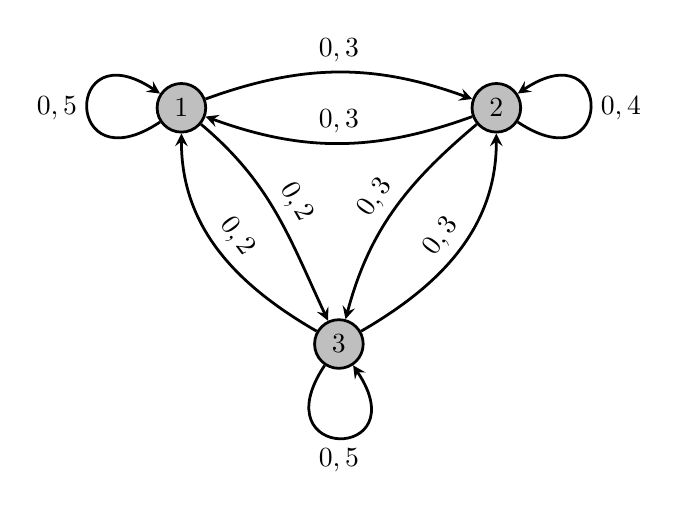
\begin{tikzpicture}[scale=1]
\tikzstyle{every path}=[>=stealth,->,line width=1pt];
\node [draw,circle,fill=gray!50] (A) at (0,0) {1};
\node [draw,circle,fill=gray!50] (B) at (4,0) {2};
\node [draw,circle,fill=gray!50] (C) at (2,-3) {3};
\draw[->] (A) to [out=20,in=160]  node[midway,sloped,above] {$0,3$}(B);
\draw[->] (A) to [out=-40,in=115]  node[midway,sloped,above] {$0,2$}(C);
\draw[->] (B) to [out=-160,in=-20] node[midway,sloped,above] {$0,3$} (A);
\draw[->] (B) to [out=-140,in=75] node[midway,sloped,above] {$0,3$} (C);
\draw[->] (C) to [out=150,in=-90] node[midway,sloped,above] {$0,2$} (A);
\draw[->] (C) to [out=30,in=-90] node[midway,sloped,above] {$0,3$} (B);
\draw[->] (B) .. controls +(1.5,-1) and +(1.5,1) .. node[midway,right]{$0,4$} (B) ;
\draw[->] (A) .. controls +(-1.5,-1) and +(-1.5,1) .. node[midway,left]{$0,5$} (A) ;
\draw[->] (C) .. controls +(-1,-1.5) and +(1,-1.5) .. node[midway,below]{$0,5$} (C) ;
\end{tikzpicture}
\end{center}

\section{Exemples en ligne}

\begin{info}
On retrouve énormément de figures créées avec TikZ sur le site \href{http://www.texample.net/tikz/examples/}{texample.net}.
\end{info}

%%%%%%%%%%%%%%%%%%%%%%%%%%%%%%%%%%%%%%%%%%%%%%%%%%%%%%%%%%%%
%%%%%%%%%%%%%%%%%%%%%%%%%%%%%%%%%%%%%%%%%%%%%%%%%%%%%%%%%%%%

\section{Exemples de figures utilisant TkZ}

%%%%%%%%%%%%%%%%%%%%%%%%%%%%%%%%%%%%%%%%%%%%%%%%%%%%%%%%%%%%
%%%%%%%%%%%%%%%%%%%%%%%%%%%%%%%%%%%%%%%%%%%%%%%%%%%%%%%%%%%%

\begin{info}
Les \jargon{packages} \ordi{TikZ} et \ordi{TkZ} sont compatibles et leurs commandes peuvent donc être utilisées pour une même figure.
\end{info}

Voici une figure du plan toute simple avec des angles marqués.

\VerbatimInput[label={[Avec des angles marqués]},gobble=0]{exemples/tkzanglesmarques.tex}

\medskip
\begin{center}
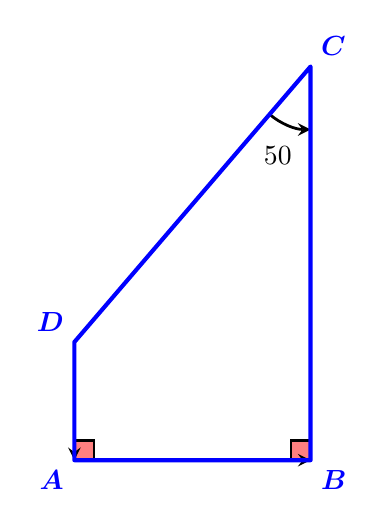
\begin{tikzpicture}[scale=1]
\tkzDefPoint(0,0){A}\tkzLabelPoints[font=\boldmath,below left,color=blue](A)
\tkzDefPoint(3,0){B}\tkzLabelPoints[font=\boldmath,below right,color=blue](B)
\tkzDefPoint(3,5){C}\tkzLabelPoints[font=\boldmath,above right,color=blue](C)
\tkzDefPoint(0,1.5){D}\tkzLabelPoints[font=\boldmath,above left,color=blue](D)
\tkzMarkRightAngle[fill=red!50](B,A,D)
\tkzMarkRightAngle[fill=red!50](C,B,A)
\tkzMarkAngle[fill=red!50,size=0.8cm](D,C,B)
\tkzLabelAngle[pos=1.2](D,C,B){50\degres}
\tkzDrawPolygon[line width=1.5pt,color=blue](A,B,C,D)
\end{tikzpicture}
\end{center}
\medskip

Voici une figure correspond au patron d'un prisme droit et sur laquelle on a marqué des angles droits, des segments de même longueur, des arcs de cercle.

\VerbatimInput[label={[Avec des arcs de cercle]},gobble=0]{exemples/tkzarccercle.tex}

\medskip
\begin{center}
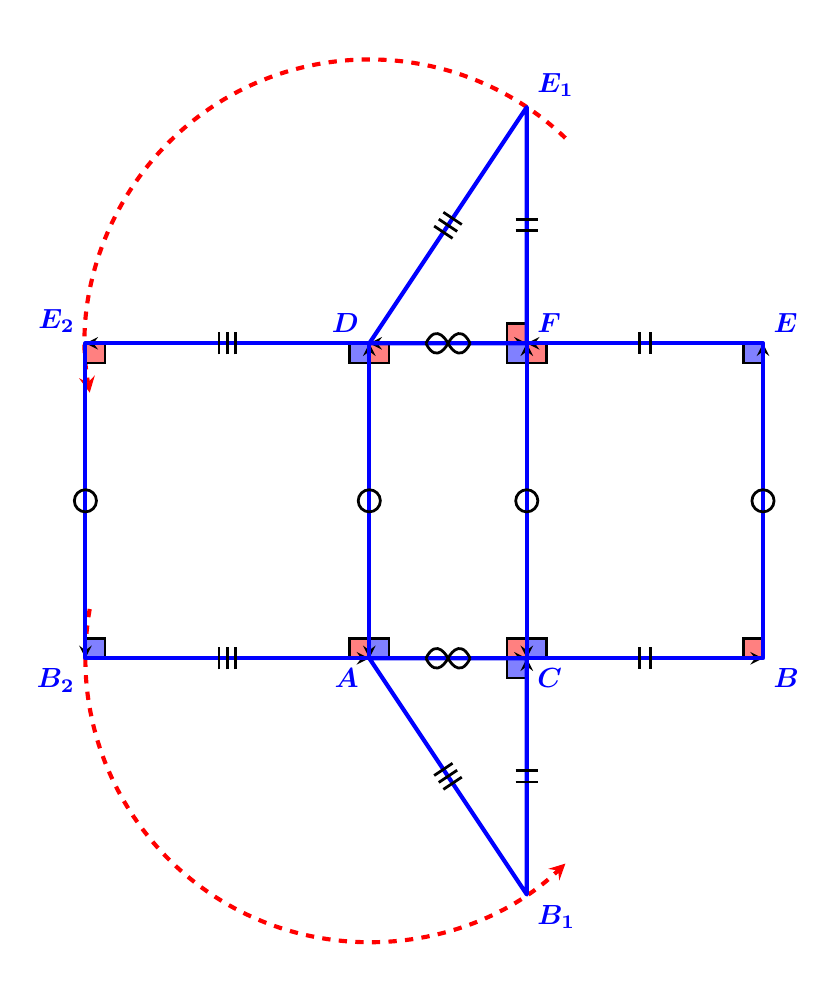
\begin{tikzpicture}[scale=1]

\tkzDefPoint(0,0){A}\tkzLabelPoints[font=\boldmath,below left,color=blue](A)
\tkzDefPoint(2,0){C}\tkzLabelPoints[font=\boldmath,below right,color=blue](C)
\tkzDefPoint(5,0){B}\tkzLabelPoints[font=\boldmath,below right,color=blue](B)
\tkzDefPoint(0,4){D}\tkzLabelPoints[font=\boldmath,above left,color=blue](D)
\tkzDefPoint(2,4){F}\tkzLabelPoints[font=\boldmath,above right,color=blue](F)
\tkzDefPoint(5,4){E}\tkzLabelPoints[font=\boldmath,above right,color=blue](E)
\tkzDefPoint(2,7){E_1}\tkzLabelPoints[font=\boldmath,above right,color=blue](E_1)
\tkzDefPoint(2,-3){B_1}\tkzLabelPoints[font=\boldmath,below right,color=blue](B_1)

\tkzCalcLength[cm](A,B_1)\tkzGetLength{dAB}

\tkzDefPoint(-\dAB,0){B_2}\tkzLabelPoints[font=\boldmath,below left,color=blue](B_2)
\tkzDefPoint(-\dAB,4){E_2}\tkzLabelPoints[font=\boldmath,above left,color=blue](E_2)

\tkzDrawArc[delta=10,line width=1.5pt,color=red,style=dashed](A,B_2)(B_1)
\tkzDrawArc[delta=10,line width=1.5pt,color=red,style=dashed](D,E_1)(E_2)

\tkzMarkRightAngle[fill=red!50](E_1,F,D)
\tkzMarkRightAngle[fill=red!50](F,C,A)
\tkzMarkRightAngle[fill=red!50](A,D,F)
\tkzMarkRightAngle[fill=red!50](D,A,B_2)
\tkzMarkRightAngle[fill=red!50](B_2,E_2,D)
\tkzMarkRightAngle[fill=red!50](C,F,E)
\tkzMarkRightAngle[fill=red!50](E,B,C)

\tkzMarkRightAngle[fill=blue!50](D,F,C)
\tkzMarkRightAngle[fill=blue!50](A,C,B_1)
\tkzMarkRightAngle[fill=blue!50](C,A,D)
\tkzMarkRightAngle[fill=blue!50](E_2,D,A)
\tkzMarkRightAngle[fill=blue!50](A,B_2,E_2)
\tkzMarkRightAngle[fill=blue!50](B,C,F)
\tkzMarkRightAngle[fill=blue!50](F,E,B)

\tkzDrawPolygon[line width=1.5pt,color=blue](B_2,A,D,E_2)
\tkzDrawPolygon[line width=1.5pt,color=blue](A,C,F,D)
\tkzDrawPolygon[line width=1.5pt,color=blue](C,B,E,F)
\tkzDrawPolygon[line width=1.5pt,color=blue](A,C,B_1)
\tkzDrawPolygon[line width=1.5pt,color=blue](D,F,E_1)

\tkzMarkSegments[mark=||,size=4pt](B_1,C C,B F,E F,E_1)
\tkzMarkSegments[mark=o,size=4pt](E_2,B_2 A,D C,F B,E)
\tkzMarkSegments[mark=|||,size=4pt](A,B_1 A,B_2 D,E_1 D,E_2)
\tkzMarkSegments[mark=oo,size=8pt](A,C D,F)


\end{tikzpicture}
\end{center}
\medskip

Voici une figure dans laquelle on définit des points comme intersection de droites et comme barycentre d'autres points.

\VerbatimInput[label={[Intersection de droites, barycentre]},gobble=0]{exemples/tkzintersectionbarycentre.tex}

\medskip
\begin{center}
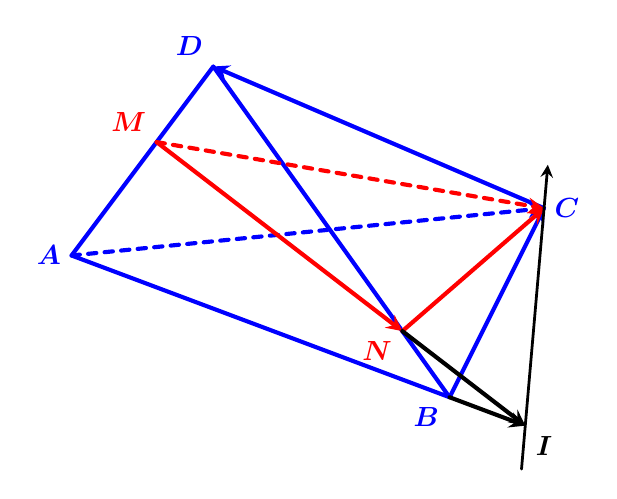
\begin{tikzpicture}[scale=0.6]

\tkzDefPoint(0,0){A}\tkzLabelPoints[font=\boldmath,left,color=blue](A)
\tkzDefPoint(10,1){C}\tkzLabelPoints[font=\boldmath,right,color=blue](C)
\tkzDefPoint(8,-3){B}\tkzLabelPoints[font=\boldmath,below left,color=blue](B)
\tkzDefPoint(3,4){D}\tkzLabelPoints[font=\boldmath,above left,color=blue](D)

\tkzDrawPolygon[line width=1.5pt,color=blue](A,B,D)

\tkzDrawSegments[line width=1.5pt,color=blue,style=dashed](A,C)

\tkzDrawSegments[line width=1.5pt,color=blue](B,C C,D)

\tkzDefBarycentricPoint(D=1,B=4)\tkzGetPoint{N}
\tkzLabelPoints[font=\boldmath,below left,color=red](N)
\tkzDefBarycentricPoint(D=3,A=2)\tkzGetPoint{M}
\tkzLabelPoints[font=\boldmath,above left,color=red](M)

\tkzInterLL(A,B)(M,N)\tkzGetPoint{I}
\tkzLabelPoints[font=\boldmath,below right](I)

\tkzDrawSegments[line width=1.5pt,color=red](M,N N,C)
\tkzDrawSegments[line width=1.5pt,color=red,style=dashed](M,C)

\tkzDrawSegments[line width=1.5pt](N,I B,I)
\tkzDrawLine[line width=1pt](I,C)

\end{tikzpicture}
\end{center}
\medskip

Voici une figure avec des vecteurs.

\VerbatimInput[label={[Avec des vecteurs]},gobble=0]{exemples/tkzvecteurs.tex}

\medskip
\begin{center}
\begin{tikzpicture}[scale=2,>=stealth]
\tkzInit[xmin=-2,xmax=5,ymin=-2,ymax=4]
\tkzGrid
\tkzDefPoint(2,3){A}\tkzDefPoint(4,2){B}
\tkzDefPointWith[orthogonal,K=-2](A,B)\tkzGetPoint{C}%AC=2*AB et (AB,AC)=-pi/2
\tkzDefPointWith[linear,K=2/3](A,C)\tkzGetPoint{D}%\vect{AD}=2/3*\vect{AC}
\tkzDefPointWith[colinear=at B,K=1/2](A,C)\tkzGetPoint{E}%\vect{BE}=1/2\vect{AC}
\tkzDrawPoints[shape=cross out,color=red,size=16pt](A,B,C)
\tkzDrawPoints[shape=cross,color=red,size=16pt](D)
\tkzDrawPoints[color=red,size=16pt](E)
\tkzLabelPoints[above right=3pt,font=\boldmath](A,B,C,D)
\tkzLabelPoints[below right=3pt,font=\boldmath,color=blue](E)
\tkzDrawSegment[->,color=blue,line width=1.5pt](B,E)
\end{tikzpicture}
\end{center}
\medskip

Voici un polygone d'effectifs cumulés croissants.

\VerbatimInput[label={[Polygone d'E.C.C.]},gobble=0]{exemples/tkzecc.tex}

\medskip
\begin{center}
\begin{tikzpicture}[scale=0.65,>=stealth]
\tkzInit[xmin=14.90,xmax=15.10,xstep=0.01,ymin=0,ymax=500,ystep=50]
\tkzGrid
\tkzDrawX[line width=1.5pt,color=blue,below right,label=Diamètres,>=stealth]
\tkzLabelX[label options={below=12pt,rotate=-45}]
\tkzDrawY[line width=1.5pt,color=blue,above left,label=E.C.C.,>=stealth]
\tkzLabelY[label options={left=6pt}]
\tkzDefPoint(14.9,0){A}
\tkzDefPoint(14.92,5){B}
\tkzDefPoint(14.94,42){C}
\tkzDefPoint(14.96,106){D}
\tkzDefPoint(14.98,204){E}
\tkzDefPoint(15,329){F}
\tkzDefPoint(15.02,431){G}
\tkzDefPoint(15.04,479){H}
\tkzDefPoint(15.06,493){I}
\tkzDefPoint(15.08,498){J}
\tkzDefPoint(15.1,500){K}
\tkzDrawPoints[color=red,size=4pt](B,C,D,E,F,G,H,I,J,K)
\tkzDrawSegments[color=red,line width=1.5pt](A,B B,C C,D D,E E,F F,G G,H H,I I,J J,K)
%Médiane
\tkzDefPoint(14.9,250){L}
\tkzDefPoint(14.9874,250){M}
\tkzDefPoint(14.9874,0){N}
\tkzDrawSegment[color=OliveGreen,line width=1.5pt,style=dashed](L,M)
\tkzDrawSegment[->,>=stealth,color=OliveGreen,line width=1.5pt,style=dashed](M,N)
\tkzText[below=30pt,color=OliveGreen](N){Med}
%1er quartile
\tkzDefPoint(14.9,125){R}
\tkzDefPoint(14.9639,125){S}
\tkzDefPoint(14.9639,0){T}
\tkzDrawSegment[color=OliveGreen,line width=1.5pt,style=dashed](R,S)
\tkzDrawSegment[->,>=stealth,color=OliveGreen,line width=1.5pt,style=dashed](S,T)
\tkzText[below=30pt,color=OliveGreen](T){$Q_1$}
%3eme quartile
\tkzDefPoint(14.9,375){U}
\tkzDefPoint(15.009,375){V}
\tkzDefPoint(15.009,0){W}
\tkzDrawSegment[color=OliveGreen,line width=1.5pt,style=dashed](U,V)
\tkzDrawSegment[->,>=stealth,color=OliveGreen,line width=1.5pt,style=dashed](V,W)
\tkzText[below=30pt,color=OliveGreen](W){$Q_3$}
\end{tikzpicture}
\end{center}
\medskip

Voici une figure construite sur un quadrillage Seyes avec des vecteurs.

Cette figure utilise une commande qui a été créée dans le preambule et qui est la suivante :

\begin{verbatim}
\newcommand{\quadrillageSeyes}[2]
{\draw[line width=0.3mm, color=blue!10, ystep=0.2, xstep=0.8] #1 grid #2;
\draw[line width=0.3mm, color=blue!30, xstep=0.8, ystep=0.8] #1 grid #2; }
\end{verbatim}

\VerbatimInput[label={[Quadrillage Seyes et vecteurs]},gobble=0]{exemples/tkzseyes.tex}

\medskip
\begin{center}
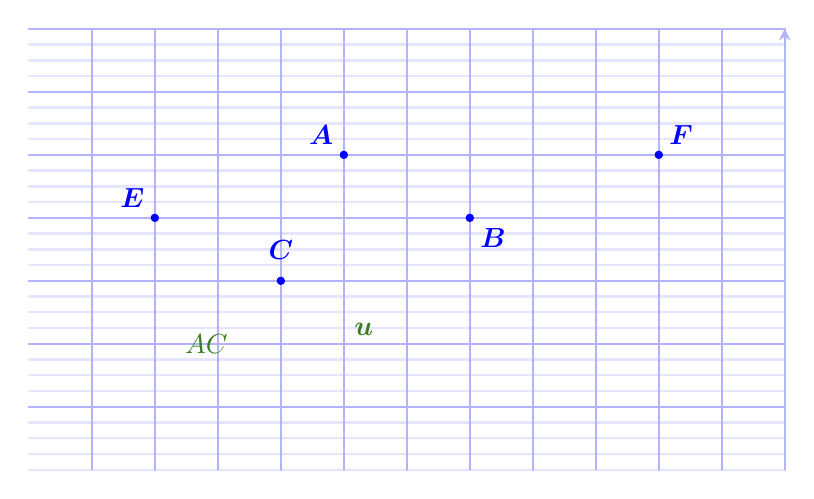
\begin{tikzpicture}
[line width=0.3mm, >=stealth, x=1cm, y=1cm,line cap=round, line join=round, scale=1]
\quadrillageSeyes{(-3.2,-2.4)}{(6.4,3.2)} 
\tkzDefPoint(0.8,1.6){A}\tkzLabelPoints[font=\boldmath,above left,color=blue](A)
\tkzDefPoint(2.4,0.8){B}\tkzLabelPoints[font=\boldmath,below right,color=blue](B)
\tkzDefPoint(0,0){C}\tkzLabelPoints[font=\boldmath,above=4pt,color=blue](C)
\tkzDefPointWith[colinear=at C,K=1](B,A)\tkzGetPoint{E}%\vect{CE}=\vect{BA}
\tkzLabelPoints[font=\boldmath,above left,color=blue](E)
\tkzDefPointWith[colinear=at B,K=1](C,B)\tkzGetPoint{F}%\vect{BF}=\vect{CB}
\tkzLabelPoints[font=\boldmath,above right,color=blue](F)
\tkzDrawPoints[size=2,color=blue](A,B,C,E,F)
\tkzDrawVectors[color=blue,line width=1.5pt,>=stealth](C,E B,A)
\tkzDrawVectors[color=red,line width=1.5pt,>=stealth](B,F C,B)

\tkzDefPointWith[colinear=at C,K=1](A,C)\tkzGetPoint{G}%\vect{CG}=\vect{AC}
\tkzDrawVectors[color=OliveGreen,line width=1.5pt,style=dotted,>=stealth](B,C C,G)
\tkzDrawVector[color=OliveGreen,line width=1.5pt,>=stealth](B,G)
\tkzLabelSegment[below right,color=OliveGreen,font=\boldmath](B,G){$\vect{u}$}
\tkzLabelSegment[left=4pt,color=OliveGreen](C,G){$\vect{AC}$}

\end{tikzpicture}
\end{center}
\medskip


Voici un graphique comportant des tangentes et un effet loupe.

Pour l'effet loupe, la librairie \jargon{spy} de TikZ a besoin d'être chargée.

\VerbatimInput[label={[Tangentes et effet loupe]},gobble=0]{exemples/tkztangenteloupe.tex}

\medskip
% requires \usetikzlibrary{spy}

\begin{center}
\begin{tikzpicture}[scale=1,spy using outlines={circle, magnification=3, connect spies}]
\tkzInit[xmin=-6,xmax=9,ymin=-2,ymax=8]
\tkzGrid[sub,subxstep=0.5,subystep=0.5]
\tkzAxeXY[>=stealth,color=blue,line width=1.5pt]
\tkzClip
%Courbe de la fonction
\tkzFct[color=red,samples=200,line width=1.5pt]
{(\x**3+\x**2-4*\x+5)/(2*\x**2-8*\x+10)}
\tkzDefPoint(7,7){F}
\tkzText[font=\boldmath,color=red,below right](F){$\calig{C}_f$}

%Points du graphique
\tkzDefPoint(0,0.5){A}\tkzLabelPoints[font=\bfseries,above right,color=blue](A)
\tkzDefPoint(2.5,6.75){B}\tkzLabelPoints[font=\bfseries,left,color=blue](B)
\tkzDrawPoints[size=4,color=red](A,B)

%Tangentes tracées
\tkzDefPoint(3,8){C}
\tkzDefPointWith[linear,K=2](C,B)\tkzGetPoint{G}%\vect{CG}=2*\vect{CB}
\tkzDrawSegment[<->,>=stealth,line width=1.5pt](C,G)
\tkzDefPoint(-1.5,0.5){D}
\tkzDefPoint(1.5,0.5){E}
\tkzDrawSegment[<->,>=stealth,line width=1.5pt](D,E)

%effet loupe
\tkzDefPoint(6,3){magnifyglass}
\spy [blue, size=5cm] on (B) in node[fill=white] at (magnifyglass);
\end{tikzpicture}
\end{center}
\medskip

\begin{info}
Avec la commande \textbackslash\verb!tkzfct!, utilisée dans l'exemple précédent, on peut tracer des courbes de fonctions avec une syntaxe relativement simplifiée.
\end{info}

Voici d'autres exemples :

\VerbatimInput[label={[Aire entre deux courbes]},gobble=0]{exemples/tkzaireentrecourbes.tex}

\medskip
\begin{center}
\begin{tikzpicture}[scale=1.25]
\tkzInit[ymin=-1,xmax=5,ymax=3]
\tkzGrid
%\tkzAxeXY
\tkzDrawX[line width=2pt,color=blue,below right,>=stealth]%,label=Rang année]
\tkzLabelX%[label options={below=12pt,rotate=-45}]
\tkzDrawY[line width=2pt,color=blue,above left,>=stealth]%,label=Montant (en \euro)]
\tkzLabelY[label options={left=6pt}]
\tkzFct[domain = 0.5:5,line width=2pt,color=red]{1/x}% courbe a
\tkzFct[domain = 1:5,line width=2pt,color=OliveGreen]{log(x)}% courbe b
\tkzDrawAreafg[between=b and a,
color=magenta!50,
domain = 1:4]
\end{tikzpicture}
\end{center}
\medskip

Visualisation d'une somme de Riemann.

\VerbatimInput[label={[Une somme de Riemann]},gobble=0]{exemples/tkzsommeriemann.tex}

\medskip
\begin{center}
\begin{tikzpicture}[scale=0.9]
\tkzInit[xmin=-3,xmax=6,ymin=-2,ymax=14,ystep=2]
\tkzDrawX \tkzDrawY
\tkzFct[line width=2pt,color = red, domain =-3:6]{(-\x-2)*(\x-5)}
\tkzDrawRiemannSumInf[fill=green!40,opacity=.5,interval=-1:5,number=10]
\end{tikzpicture}
\end{center}
\medskip

Une courbe paramétrée.

\VerbatimInput[label={[Une courbe paramétrée]},gobble=0]{exemples/tkzcourbeparametree.tex}

\medskip
\begin{center}
\begin{tikzpicture}[scale=1.25]
\tkzInit[xmin=-50,xmax=50,xstep=10,
ymin=-50,ymax=50,ystep=10]
\tkzGrid
\tkzDrawX[line width=2pt,color=blue,below right,>=stealth]
\tkzLabelX%[label options={below=12pt,rotate=-45}]
\tkzDrawY[line width=2pt,color=blue,above left,>=stealth]
\tkzLabelY[label options={left=6pt}]
\tkzFctPar[color=red,line width=2pt,smooth,samples=200,domain=0:50]{t*sin(t)}{t*cos(t)}
\end{tikzpicture}
\end{center}
\medskip

Des aires sous une courbe.

\VerbatimInput[label={[Des aires sous une courbe]},gobble=0]{exemples/tkzairesouscourbe.tex}

\medskip
\begin{tikzpicture}[scale=1.75]
\tkzInit[xmin=0,xmax=800,xstep=100,
ymin=0,ymax=2000,ystep=400]
\tkzGrid
\tkzDrawX[line width=2pt,color=blue,below right,>=stealth]
\tkzLabelX%[label options={below=12pt,rotate=-45}]
\tkzDrawY[line width=2pt,color=blue,above left,>=stealth]
\tkzLabelY[label options={left=6pt}]
\tkzFct[domain = 0:800]{(1./90000)*\x*\x*\x-(1./100)*\x*\x+(113./36)*\x}
\tkzDefPoint(450,400){a}
\tkzDrawArea[color=blue!50, domain =0:450]
\tkzDrawArea[color=red!50, domain =450:800]
\tkzDrawPoint[size=4pt](a)
\end{tikzpicture}

%\medskip

